\chapter{KMS - \textit{Kubernetes Micro Scheduler}\label{cap-proposta}}

Este capítulo tem como objetivo apresentar os processos de desenvolvimento do escalonador distribuído proposto, denominado \ac{KMS}. A escolha do nome está concentrada na etimologia da palavra \textbf{micro}, a qual significa \textbf{pequeno}, visto que um dos principais objetivos do presente trabalho é distribuir o escalonador utilizando conceitos de \textbf{micro}sserviços. Ou seja, fragmentar um escalonador monolítico em pequenos sistemas que operam de forma independentes, mas em conjunto refletem um sistema distribuído robusto.

No início do capítulo é apresentado um comparativo entre o \ac{KMS} com as atuais abordagens de escalonamento do \textit{Kubernetes}, o principal objetivo nesta seção é confrontar as arquiteturas em cenários de falhas. Ao passo que, as seções subsequentes são dedicadas ao funcionamento dos componentes do \ac{KMS}, como também as trocas de mensagens. Exceto a Seção 3.2, que é destinada à apresentar a documentação baseada na engenharia de requisitos para delimitar o escopo do projeto.

%O presente trabalho visa o desenvolvimento de um escalonador distribuído, baseado em microsserviços, e a sua implantação no \textit{Kubernetes}. Dessa forma, os principais objetivos do escalonador proposto são ampliar a escalabilidade visando otimizar as métricas de tempo de espera de escalonamento e \textit{makespan}, como também tratar as falhas de forma competente.

%O desafio inicial é a identificação dos microsserviços a partir de uma abordagem fundamentada em sistemas distribuídos. O segundo desafio é relacionado ao desenvolvimento do projeto, o qual será visado um sistema documentado, consistente e tolerante a falhas, alcançados por meio de uma arquitetura robusta e replicável. O terceiro desafio compreende na implantação da solução para o \textit{Kubernetes}, como também os resultados a partir das métricas de interesse.

\section{Comparativo com abordagem padrão do \textit{Kubernetes}}
A visualização da proposta e do desempenho esperado do escalonador proposto é notável ao ser comparado com as demais abordagens de escalonamento que o \textit{Kubernetes} oferece (com e sem réplica do \textit{node master)}, como esboça a Figura \ref{fig:comp_sched}.

A figura representa o comportamento de três métodos de escalonamento de contêineres: Escalonador padrão \textit{Kubernetes} com \textit{(1)} e sem \textit{(2)} réplica e o escalonador distribuído proposto \textit{(3)} em um período de tempo dividido em eventos de escalonamento. No primeiro evento de escalonamento há uma solicitação de 100\% de uso dos recursos, e em todas as abordagens o escalonamento é executado com sucesso, pois os recursos estavam disponíveis e não ocorreram falhas. No segundo evento há uma nova solicitação que consome 50\% dos recursos, entretanto, houve a simulação de uma falha do tipo \textit{crash}. Por conta disso, a abordagem \textit{(1)} utilizará um evento de escalonamento para reinicialização do sistema e a abordagem \textit{(2)} redirecionará as requisições para a réplica de escalonamento. Diferente disso, o escalonador distribuído \textit{(3)} é capaz de executar o escalonamento parcial, dado que a falha ocorreu em apenas uma unidade do sistema distribuído. A principal consequência no comportamento do escalonador \textit{(1)} e \textit{(2)} é no atraso das requisições em efeito cascata. Por consequência, todas as requisições que excedem a capacidade de recursos são atrasadas para o próximo passo de escalonamento, causando degradamento do tempo de espera e \textit{slowdown}.

\begin{figure}[h!]
	\caption{\label{fig:comp_sched}Comparação das abordagens de escalonamento}
	\centering
	% \includegraphics[width=\linewidth]{figuras/schedule-proposal.png}
	% \hspace*{-.85in}
	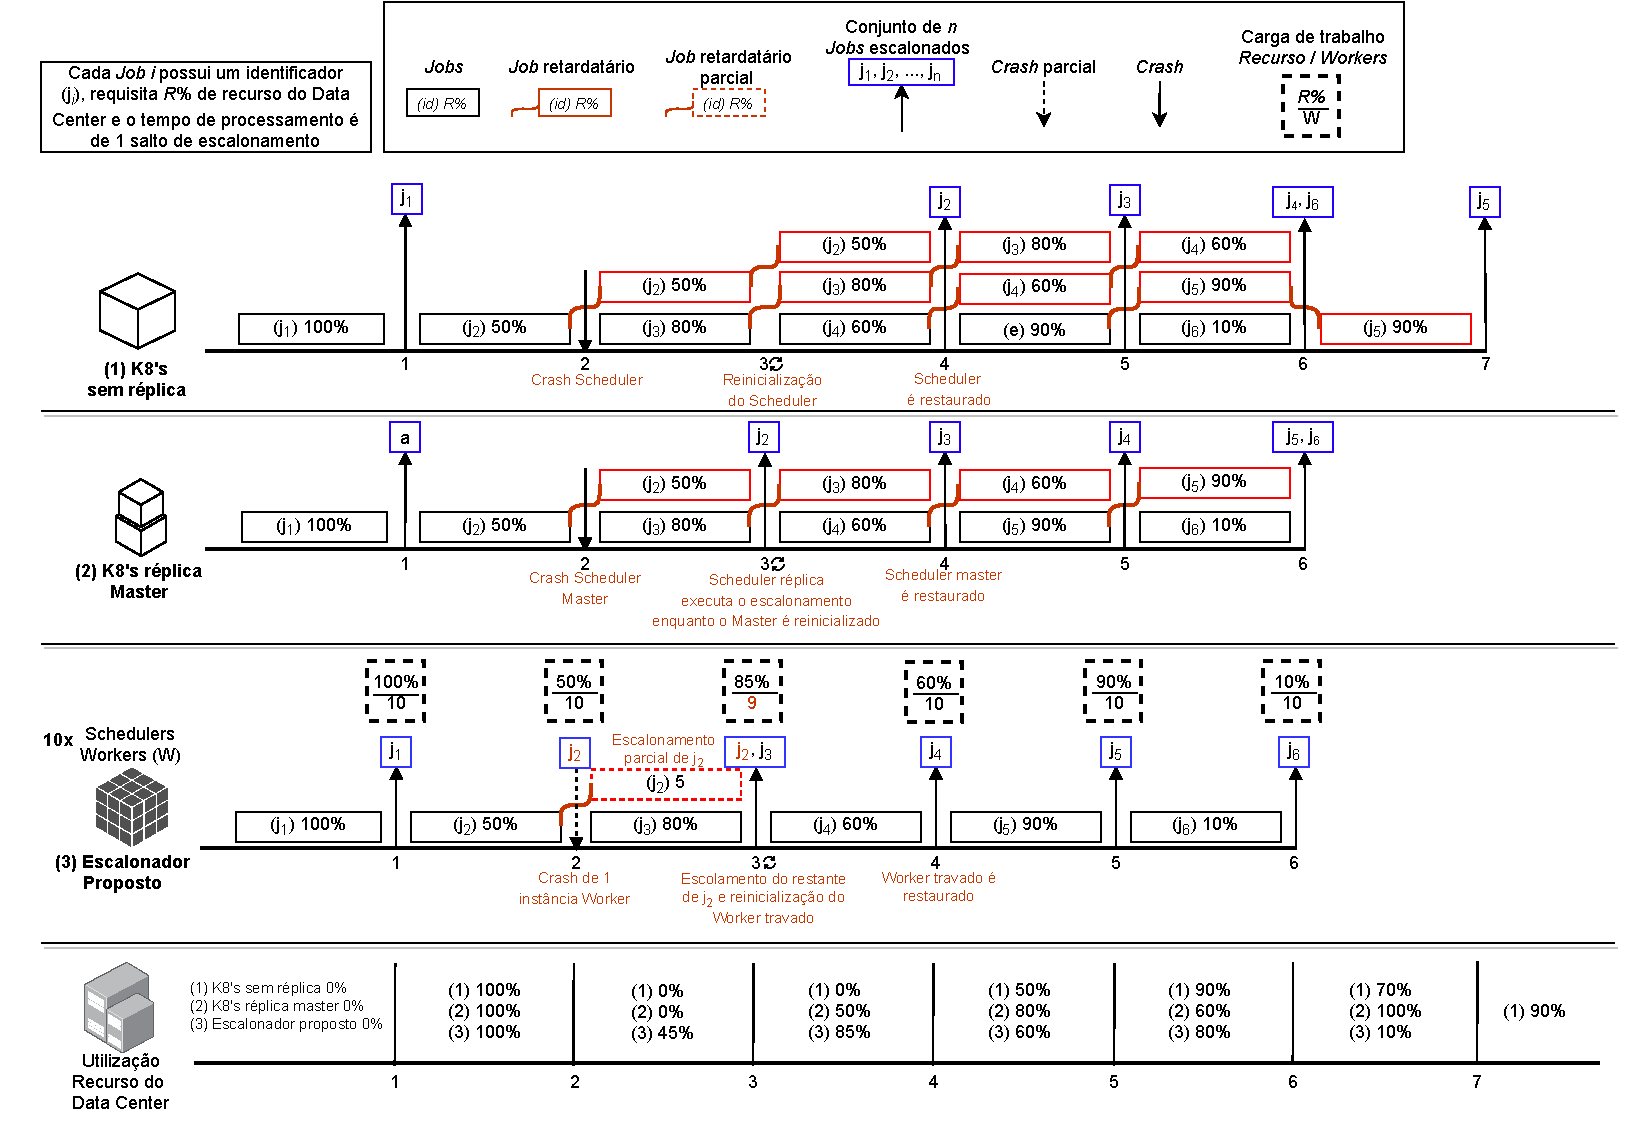
\includegraphics[width=1\linewidth]{assets/schedule-proposal.drawio.pdf}
	\legend{Fonte: O autor}
\end{figure}



\section{Levantamento de Requisitos}

Nessa seção objetiva-se desenvolver uma documentação compreensível do sistema distribuído proposto guiado pela engenharia de requisitos. O levantamento de requisitos é o passo inicial para entendimento do escopo e objetivos do \ac{KMS}, foi desenvolvido utilizando a técnica de análise de cenário e objetivos desejados. No contexto do presente trabalho, buscou-se elencar os requisitos funcionais a partir do comportamento do sistema distribuído e suas funcionalidades, já os requisitos não funcionais aqueles que representam as propriedades e restrições desejadas. 

\subparagraph{Requisitos funcionais}
\begin{enumerate}
	\item Escalonar cargas de trabalho utilizando arquitetura hierárquica de sistemas distribuídos, denominada \textit{master/worker};
	\item Particionar o \textit{cluster}. Cada partição será gerenciado por um escalonador dedicado denominado \textit{worker};
	\item \textit{Workers} serão responsáveis por escalonar cargas de trabalhos nos segmentos do \textit{cluster};
	\item Implementação de estratégias de escalonamento conhecidas na literatura, como por exemplo: \textit{Round-Robin}, \textit{Binpack} e \textit{Easy Backfiling}; e
	\item Possibilidade de intercambiar o algoritmo de escalonamento.
\end{enumerate}

\subparagraph{Requisitos não funcionais}
\begin{enumerate}
	\item O escalonador deverá ser compatível com o \textit{Kubernetes};
	\item Executar os microsserviços virtualizados em contêineres;
	\item O sistema não deve conter único ponto de falha, todos os componentes deverão ser distribuídos;
	\item Desenvolver os principais componentes (\textit{Master} e \textit{Worker}) no formato de microsserviços \textit{stateless}.
	\item Desenvolver um sistema distribuído de forma transparente, ou seja, promover acesso aos recursos distribuídos de forma oculta, como se fosse um único sistema para o usuário; e
	\item Utilizar a estratégia de múltiplos escalonadores, como discutido na seção 2.2.4.
\end{enumerate}

\section{Identificação dos Componentes}

Em síntese, o \ac{KMS} consiste em um modelo hierárquico de sistema distribuído, possuindo 2 componentes principais: \textit{Master} e \textit{Worker}. O componente \textit{Master} corresponde ao único ponto de centralização, isso não significa que haverá um único ponto de falha no sistema, mas sim que este componente manterá apenas uma instância ativa executando o trabalho dentre todas as suas réplicas. Ao fazer uma analogia com a arquitetura Produtor/Consumidor, o componente \textit{Worker} corresponde ao Consumidor, pois é responsável por executar as ações de escalonamento do \ac{KMS}, enquanto que o \textit{Master} é interpretado como Produtor, em razão de lidar com a delegação de trabalho.


% Baseado em um modelo hierárquico, o sistema distribuído proposto consiste em dois componentes principais: \textit{master} e \textit{worker}. O componente \textit{master} corresponde ao único ponto de centralização, já o \textit{worker} é \textit{stateless} e replicável. Cada componente possui uma responsabilidade distinta e específica e em conjunto eles representam o \ac{KMS}.

\subsection{\textit{Master}}

O Master é responsável por buscar cargas de trabalho (\textit{pods}) na fila de escalonamento do \textit{Kubernetes}, em seguida distribuir as cargas para os \textit{Workers}.  Ou seja, é um componente relacionado com a delegação de trabalho, considerado o produtor em um sistema distribuído. Um dos princípios do desenvolvimento, não só do componente \textit{Master}, mas de todo o sistema, é implementar uma arquitetura modular a qual seja possível intercambiar entre as técnicas de escalonamento (seguindo os princípios DDD previamente descritos). O primeiro ponto de escalonamento é encontrado na distribuição das cargas de trabalho do \textit{Master} para os \textit{Workers}. Por exemplo, duas estratégias são observadas na Figura \ref{fig:distribuicao_cargas}: \textit{Binpack} e \textit{Spread}. \textit{Binpack} está relacionado com a minimização dos recursos, ou seja, o algoritmo selecionará o mesmo \textit{Worker} enquanto existirem recursos nessa unidade computacional - na imagem o \textit{worker$_1$} está apenas com 40\% de utilização, por isso todos os \textit{pods} estão sendo direcionados a ele. Já o \textit{Spread} possui como objetivo otimizar o balanceamento de carga dos recursos, comumente utilizado \textit{round-robin}, sendo possível notar que as cargas estão sendo distribuídas de forma igualitária entre os \textit{workers}.

\begin{figure}[h!]
	\caption{\label{fig:distribuicao_cargas} Estratégias de distribuição de cargas entre \textit{master} e \textit{workers}}
	\centering
	% \includegraphics[width=\linewidth]{figuras/schedule-proposal.png}
		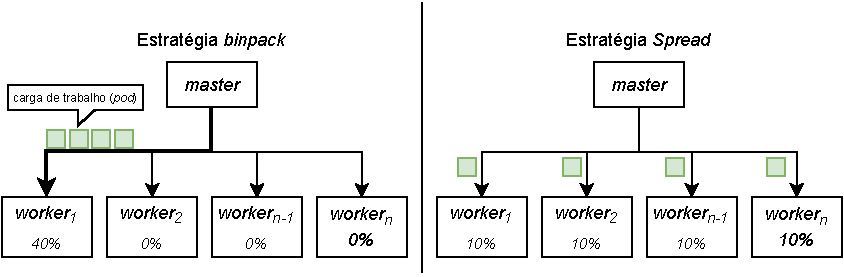
\includegraphics[width=\linewidth]{assets/distribuicao-trabalho.pdf}
	\legend{Fonte: O autor}
\end{figure}

\subsection{\textit{Worker}}

O \textit{Worker} tem como objetivo resolver o escalonamento, ou seja, encontrar um \textit{node} específico para executar o \textit{pod}. A principal característica é ser um componente \textit{stateless} - não armazena estado. Isso é possível, uma vez que foi desenvolvido no formato de microsserviço: recebe uma entrada, executa regras no escopo fechado da entrada e gera uma saída. Dessa forma, a entrada do \textit{Worker} consiste no estado atual do \textit{Cluster} e na lista de \textit{Pods}, que são informados, respectivamente, pela \textit{API} do \textit{Kubernetes} e pelo componente \textit{Master} do \ac{KMS}. Após ler a entrada são executadas operações em relação ao escalonamento, por fim, a saída representa o resultado do escalonamento.

\begin{figure}[h!]
	\caption{\label{fig:microsservico-worker} Comparativo Microsserviço x \textit{Worker}}
	\centering
	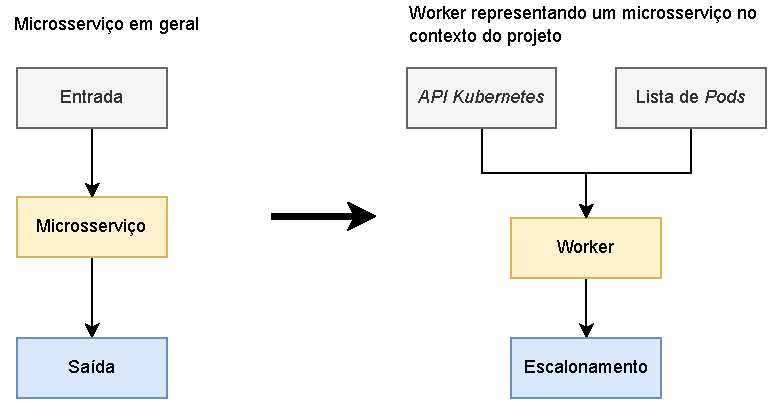
\includegraphics[width=\linewidth]{assets/microsservico-worker.pdf}
	\legend{Fonte: O autor}
\end{figure}

A Figura \ref{fig:microsservico-worker} esboça o comparativo entre entre arquitetura de microsserviço genérica com o componente \textit{Worker}. No \ac{KMS}, o \textit{Worker} é um componente com réplicas, e todas ativas. A ideia é que cada instância gerencie uma partição do \textit{cluster} \textit{Kubernetes}. Por exemplo, considere um \textit{cluster} com \textit{m} nós computacionais e \textit{w} \textit{Workers}, nesse contexto, cada instância do \textit{Worker} será responsável por $m/w$ nós do \textit{cluster}. Isto é, a instância executará o escalonamento no conjunto de nós que pertencem a sua partição.

Ao executar o \ac{KMS} em um \textit{cluster} com 6 nós computacionais e 2 instâncias do componente \textit{Worker}, o \textit{cluster} será seccionado em 2 conjuntos de nós de tamanho 3 (\textit{Tamanho Cluster} / \textit{quantidade réplicas Worker}). Logo, cada instância do \textit{Worker} será responsável por processar o escalonamento da sua respectiva partição, como demonstra a Figura \ref{fig:particionamento-worker}.
Especificamente, tanto o \textit{Worker$_0$} quanto o \textit{Worker$_1$} residem em \textit{Node$_0$}, o que deve-se ao fato que ambas as instâncias foram escalonadas pelo escalonador padrão do \textit{Kubernetes}, que tomou a decisão, neste exemplo de forma hipotética, de escalonar as duas réplicas no mesmo nó computacional. Os componentes internos do \ac{KMS} são escalonados pelo escalonador padrão do \textit{Kubernetes}.

\begin{figure}[h!]
	\caption{\label{fig:particionamento-worker} Particionamento do \textit{cluster} entre \textit{workers}}
	\centering
	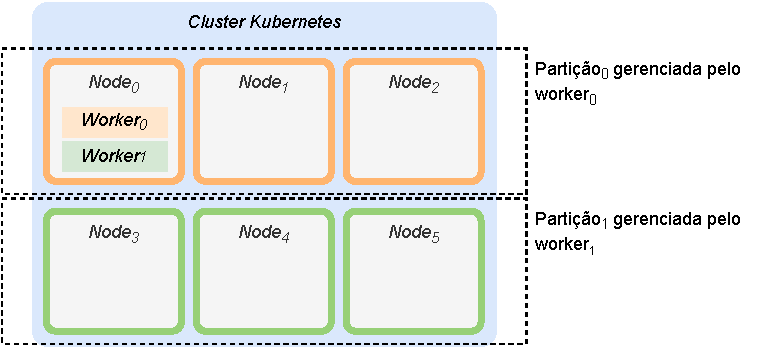
\includegraphics[width=\linewidth]{assets/particionamento-worker.pdf}
	\legend{Fonte: O autor}
\end{figure}

\subsection{Relação \textit{Master}-\textit{Worker}}
As subseções anteriores 3.3.1 e 3.3.2 se encarregaram de apresentar os componentes de forma isolada, nesta subseção objetiva-se sintetizar o funcionamento do \ac{KMS} como um todo. Aqui o principal objetivo é relacionar os componentes \textit{Master} e \textit{Worker}. Em resumo, o \ac{KMS} consiste em 3 passos objetivos: (1) Buscar os \textit{Pods} na fila de escalonamento interna do \textit{Kubernetes}, (2) Distribuir as cargas de trabalho entre os \textit{Workers} e (3) Executar o escalonamento.

%no formato de microsserviço, a ideia é que cada unidade execute o escalonamento em uma partição específica do \textit{cluster}. Dessa forma, ao se executar \textit{n} \textit{workers} então o \textit{cluster} será particionado em \textit{n} partes, como esboça a Figura \ref{fig:worker}.

%\begin{figure}[h!]
%	\caption{\label{fig:worker} particionamento do \textit{cluster} entre \textit{workers}}
%	\centering
%	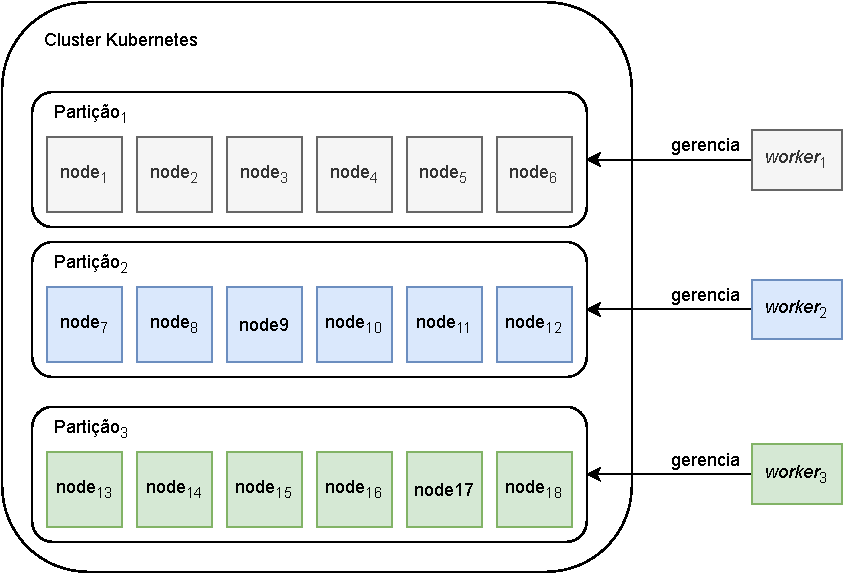
\includegraphics[width=.80\linewidth]{assets/worker.pdf}
%	\legend{Fonte: O autor}
%\end{figure}

%A comunicação entre o sistema distribuído proposto e o \textit{Kubernetes} é efetuada pelo protocolo \ac{HTTP}, em resumo, o \textit{Kubernetes} expõe um servidor \textit{Web} que pode ser consumido por qualquer componente interno. No contexto do presente trabalho, o \textit{Master} consumirá a \textit{API} para buscar os contêineres que estão na fila de escalonamento. Na mesma linha de pensamento, o componente \textit{Worker} se comunicará com a \textit{API} para enviar ordens de escalonamento. Por outro lado, a comunicação entre o componente \textit{master} e \textit{worker} será efetivada via protocolo \textit{gRPC}. Protocolo de comunicação projetado pela \textit{Google}, a principal característica é a performance de alta velocidade entre \textit{microsserviços}.
%O fluxo de execução do sistema distribuído proposto é representado pelo diagrama de fluxo esboçado pela Figura \ref{fig:flow_diagram}.

\begin{figure}[h!]
	\caption{\label{fig:relacao-master-worker}Diagrama de Fluxo}
	\centering
	% \includegraphics[width=0.3\linewidth]{figuras/schedule-proposal.png}
	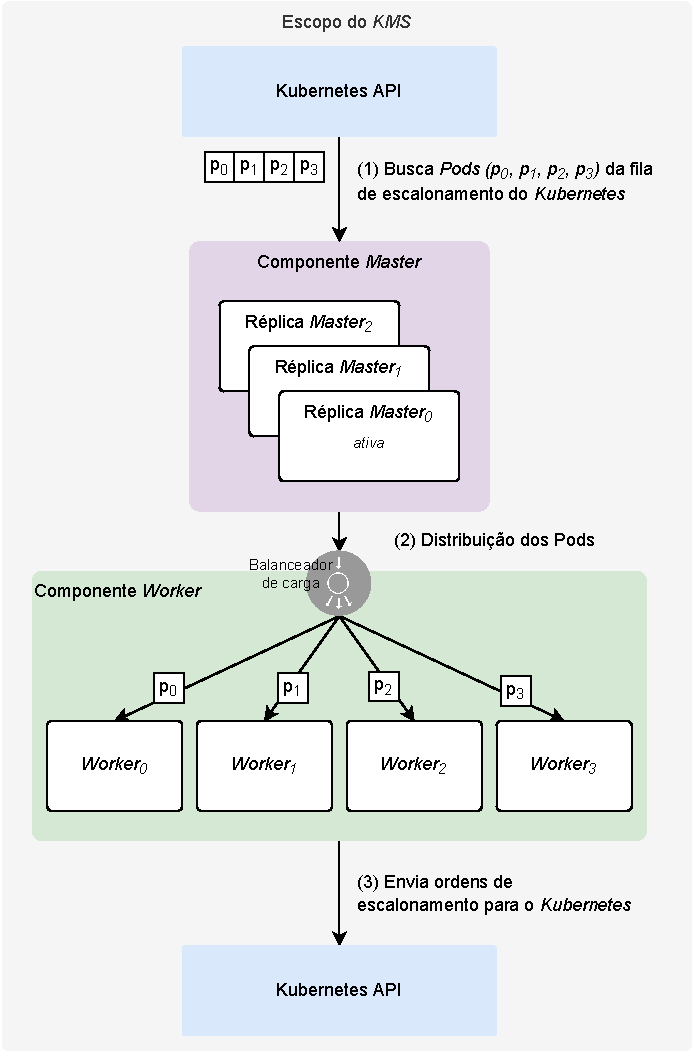
\includegraphics[width=.60\linewidth]{assets/relacao-master-worker.pdf}
	\legend{Fonte: O autor}
\end{figure}

Considerando um cenário do \ac{KMS} com 3 réplicas \textit{Master} e 4 réplicas \textit{Worker}, o funcionamento do sistema distribuído proposto pode ser visualizado na Figura \ref{fig:relacao-master-worker}. O diagrama apresenta a interação completa entre os módulos do \ac{KMS}, desde a coleta do \textit{Pod} pelo \textit{Master}, até o envio da ordem de escalonamento pelo \textit{Worker} para a \textit{API} do \textit{Kubernetes}. Além disso, é possível verificar que no topo do componente \textit{Worker} há um balanceador de carga, que é responsável por distribuir as requisições de escalonamento de \textit{Pods}. Com isso, o componente \textit{Master} não necessita guardar estado das instâncias do \textit{Worker}, uma vez que comunicar-se diretamente com o balanceador de carga é o suficiente. No \textit{Kubernetes} o balanceador de carga pode ser configurado tanto para a estratégia \textit{Binpack} quanto para \textit{Round-Robin}. No exemplo da figura, a estratégia executada foi \textit{Round-Robin}. Outro ponto de destaque são as réplicas do componente \textit{Master}, considerado o \textbf{Produtor} do sistema distribuído, as instâncias do \textit{Master} necessitam executar algoritmo de eleição para manter apenas uma ativa executando a tarefa de \textbf{Produtor}. O algoritmo de eleição será apresentado na Seção \ref{eleicao-master}.

%Na Figura \ref{fig:flow_diagram} é exemplificado o fluxo de execução da arquitetura proposta e os papéis dos dois módulos principais: \textit{master} e \textit{worker}. O \textit{master} é responsável por buscar fila de \textit{pods} não escalonados (1) -- na figura é esboçado por $p_1, p_2, p_3, p_4, p_5, p_6, p_{n-1}, p_n$ -- e também por distribuí-los (2) aos \textit{workers} -- na figura é esboçado por $w_1, w_2, w_{n-1}, w_{n}$ --, nesta etapa foi utilizado o método de espalhamento para enviar a carga de trabalho para os \textit{workers}. Entretanto, o presente trabalho busca modularizar a arquitetura proposta de forma que possibilite intercambiar a técnica de escalonamento e utilizar, por exemplo, agrupamento ou até mesmo métodos refinados. Na etapa (2) será utilizado comunicação via \textit{gRPC}.

%No \textit{worker} há duas funções principais. A primeira é o recebimento das cargas de trabalho como é notado na figura em (2). Para isso cada unidade \textit{worker} gerencia uma fila interna que representa em ordem de chegada as cargas de trabalho enviadas pelo \textit{master}. A segunda função, a principal, é a execução do algoritmo de escalonamento que vinculará o \textit{pod} a um \textit{node}. O método de escalonamento será modular, ou seja, haverá uma lista de implementações de escalonamento pré-definida (\textit{spread, binpack, backfilling}), mas o objetivo é que seja extensível e possa executar até métodos refinados de escalonamento.

\section{Trocas de Mensagens}

A comunicação entre o sistema distribuído proposto e o \textit{Kubernetes} é efetuada pelo protocolo \ac{HTTP}. Em resumo, o \textit{Kubernetes} expõe um servidor \textit{Web} que pode ser consumido por qualquer componente interno. No contexto do presente trabalho, o \textit{Master} consumirá a \textit{API} para buscar os contêineres que estão na fila de escalonamento. Na mesma linha de pensamento, o componente \textit{Worker} se comunicará com a \textit{API} para enviar ordens de escalonamento. A comunicação entre o componente \textit{Master} e \textit{Worker} também será efetivada via protocolo \ac{HTTP}, em síntese, cada instância do \textit{Worker} abrirá um servidor \textit{Web} para consumir as cargas de trabalho enviadas pelo \textit{Master}. Ao utilizar essa arquitetura, é possível definir novas rotas para o servidor \textit{Web} do \textit{Worker}, além daquelas relacionadas ao escalonamento, como por exemplo, rotas para verificar sobrecarga de recursos do contêiner (\textit{CPU} e \textit{RAM}). Para elucidar as trocas de mensagens, foi elaborado um diagrama de sequência com os eventos principais do \ac{KMS} na Figura \ref{fig:sequencia}. 

\begin{figure}[h!]
	\caption{\label{fig:sequencia}Diagrama de Sequência \ac{KMS}}
	\centering
	% \includegraphics[width=0.3\linewidth]{figuras/schedule-proposal.png}
	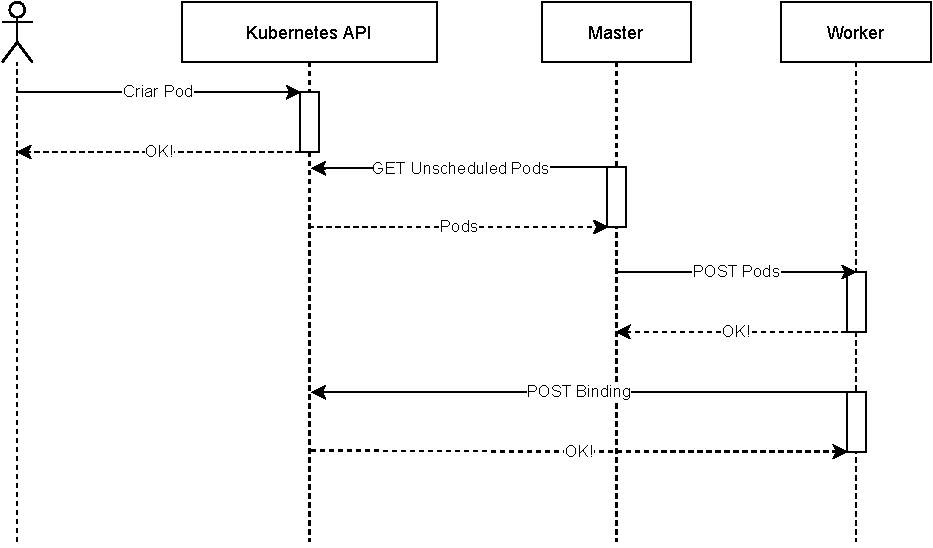
\includegraphics[width=\linewidth]{assets/sequencia.pdf}
	\legend{Fonte: O autor}
\end{figure}

Como todos os módulos do \ac{KMS} se comunicam por \textit{HTTP}, o diagrama de sequência foi elaborado utilizando a nomenclatura padrão de requisições \textit{Web} - \textit{POST e GET}. O ponto de partida é no momento em que um novo \textit{Pod} é inserido na plataforma pelo usuário, devendo ser executado obrigatoriamente pela \textit{API} do \textit{Kubernetes}, na figura corresponde ao evento \textit{Criar Pod}. O \textit{Pod} permanecerá na fila de escalonamento interna até algum escalonador requisitar os \textit{Pods} não escalonados, que é observado no evento \textit{GET Unscheduled Pods}. O próximo passo é distribuir os \textit{Pods} para os \textit{Workers} por meio do evento \textit{POST Pods}, que é executado pelo \textit{Master}. Ao fim, o \textit{Worker} executa o escalonamento e envia uma ordem do tipo \textit{binding} para a \textit{API} do \textit{Kubernetes}, que vinculará o \textit{Pod} à algum nó eleito pelo \textit{Worker} no processo de escalonamento. Essa última etapa é representada pelo evento \textit{POST binding}.


\section{Eleição do Componente \textit{Master} \label{eleicao-master}}

Um dos princípios do \ac{KMS} é desenvolver uma aplicação distribuída sem um único ponto de falha. Essa abordagem influencia que todos os módulos do sistema necessitem alguma técnica de controle de falhas. As instâncias do \textit{Worker} são considerados microsserviços e todas as sua réplicas trabalham simultaneamente no escalonamento. Entretanto, o módulo \textit{Master}, mencionado nas seções anteriores como \textbf{Produtor} do sistema distribuído, demanda que apenas uma réplica esteja ativa trabalhando no escalonamento enquanto que as outras estarão em espera. Dado o contexto, verificou-se que uma das formas de resolver este problema é utilizar algoritmo de eleição para manter apenas uma instância do \textit{Master} executando o escalonamento enquanto que o restante permanecerão em estado de espera.

Visando simplificar o desenvolvimento, as réplicas do componente \textit{Master} se comunicarão com o \textit{Redis} \cite{Redis} para executar o ambiente de eleição. Ao contrário da abordagem padrão de banco de dados relacionais, o \textit{Redis} é considerado não relacional do tipo Chave-Valor em memória. A principal utilização dessa tecnologia é no \textit{caching} de informação devido ao seu rápido acesso aos dados. Além disso, é possível utilizar com persistência em disco, transmissão em tempo real de informação (\textit{Streaming Engine}) e mensagens de inscrição em tópicos do tipo \textit{Publish/Subscribe}, em conclusão, o \textit{Redis} é uma eficiente tecnologia no desenvolvimento de sistemas distribuídos.

O principal objetivo da escolha do \textit{Redis} é se beneficiar da funcionalidade de \textit{Locks Distribuídos}. Os \textit{Locks Distribuídos} são considerados uma primitiva de banco de dados, que auxiliam em cenários nos quais diferentes processos operam recursos compartilhados de forma mutuamente exclusiva \cite{redisDistributedLocks}.

\subsection{Algoritmo de eleição apoiado no \textit{Redis}}

Em síntese, o processo de eleição, baseado em \textit{Locks Distribuídos}, consiste em reproduzir um cenário de corrida entre os processos, o primeiro que conseguir escrever a sua identificação no recurso compartilhado do \textit{Redis} será eleito líder. O recurso compartilhado é no formato de um campo Chave-Valor e possui tempo de expiração (\textit{TTL - Time to live}), o campo voltará a ser nulo no momento em que atingir a data de expiração, dessa forma, habilitando uma nova corrida entre os processos.

Para exemplificar a execução do algoritmo de eleição apoiado no \textit{Redis}, foi desenvolvido um diagrama com 6 passos. Neste exemplo, considere que há 3 réplicas do componente \textit{Master} que estarão disputando a eleição do líder. A réplica que for eleita executará o escalonamento e as regras do \textit{Master}, enquanto que as restantes permanecerão em espera por uma nova oportunidade de eleição. Os diagramas podem ser vistos na Figura \ref{fig:eleicao-todos-os-passos}.

\begin{figure}[h!]
	\caption{\label{fig:eleicao-todos-os-passos}Processos de eleição do \textit{Master}}
	\centering
	% \includegraphics[width=0.3\linewidth]{figuras/schedule-proposal.png}
	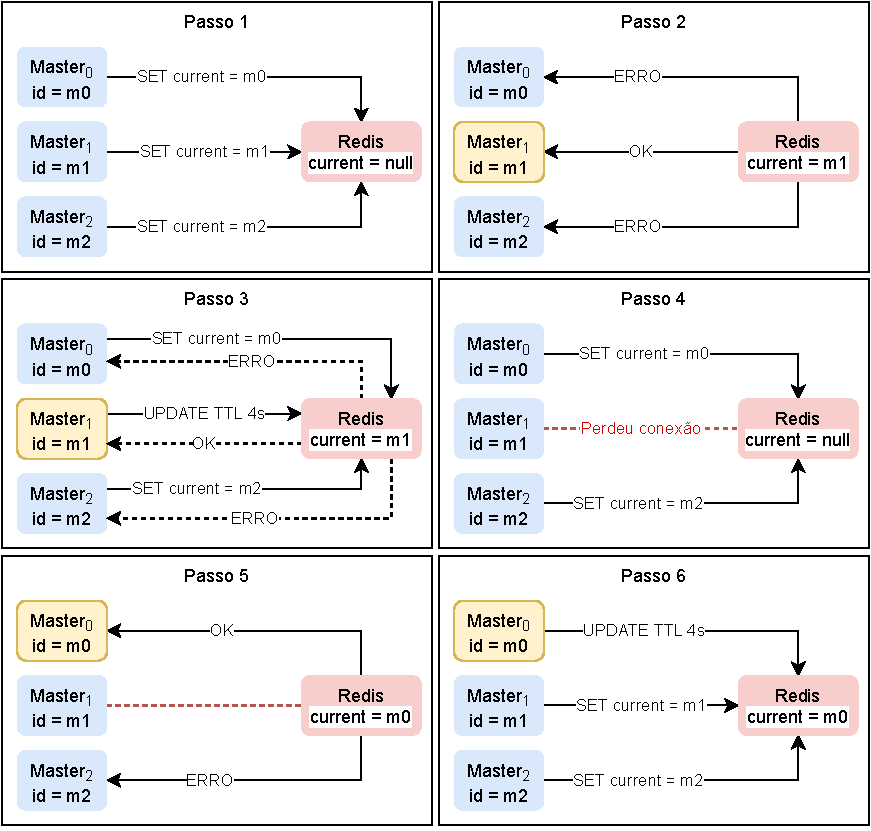
\includegraphics[width=\linewidth]{assets/eleicao-todos-os-passos.pdf}
	\legend{Fonte: O autor}
\end{figure}

\subparagraph{Passo 1:} Todos os \textit{Masters} tentarão escrever no campo \textit{current} do Redis o próprio \textit{id}. Por exemplo, \textit{Master$_2$} tentará escrever \textit{m2} em \textit{current}. O campo \textit{current} foi configurado para ser compartilhado de forma mutuamente exclusiva e possui tempo de expiração de 4 segundos.

\subparagraph{Passo 2:} \textit{Redis} vai utilizar \textit{lock} interno e apenas uma instância do \textit{Master} conseguirá escrever o id no campo \textit{current}. Só é possível escrever se o campo current for nulo. Nesse exemplo, \textit{Master$_1$} foi premiado e tornou-se líder. Neste passo, o \textit{Redis} responde com sucesso apenas o \textit{Master$_1$}.

\subparagraph{Passo 3:} O \textit{Redis} está configurado para expirar o campo \textit{current} a cada 4 segundos, assim permitindo a corrida entre os \textit{Masters}.
Ao passo que, o líder, no caso \textit{Master$_1$}, a cada intervalo de 2 segundos estenderá o \textit{TTL} do campo \textit{current} em 4 segundos.

\subparagraph{Passo 4:} Considere que o \textit{Master$_1$} perdeu a conexão ou foi derrubado. Ou seja, não irá conseguir atualizar o \textit{TTL} do valor \textit{current}. Portanto, em 4 segundos o valor \textit{current} voltará a ser nulo, dessa forma, habilitando uma nova corrida entre os \textit{Masters}.

\subparagraph{Passo 5:} Como o campo \textit{current} voltou a ser nulo, uma nova corrida é executada. Considere que o \textit{Master$_0$} conseguiu escrever \textit{m1} em \textit{current} e será o novo líder e responsável por atualizar o \textit{TTL} enquanto ainda estiver disponível.

\subparagraph{Passo 6:} Este passo representa o reinício do algoritmo, em que o último líder eleito, no caso o \textit{Master$_0$}, será responsável por atualizar o \textit{TTL} do campo \textit{current}. No momento em que não for possível atualizar, o campo voltará a ser nulo dando início uma nova corrida entre as réplicas.


\section{Implantação em \textit{Kubernetes}}
O \ac{KMS} é executado no topo do \textit{Kubernetes}, dessa forma, os componentes principais são conteinerizados e provisionados pelo próprio \textit{Kubernetes}. Na Seção 2.2.4 foram apresentadas 4 formas distintas de customizar o escalonador padrão, após analisar a viabilidade, chegou-se a conclusão que o método \textbf{Múltiplos escalonadores} é o ideal para a implementação do projeto. Essa abordagem consiste no desenvolvimento de um escalonador que é executado no formato de \textit{Pod} e toda a comunicação com o \textit{Kubernetes} é realizada via troca de mensagens por meio da \textit{API}. Com isso, o componente \textit{Worker} é considerado \textit{stateless}, pois as suas dependências (estado do \textit{cluster} e a lista de \textit{Pods} não escalonados) são considerados parâmetros. Neste contexto, o problema de escalonamento, na visão do \textit{Worker}, é da forma entrada e saída: a entrada é o estado do \textit{cluster} que é informado pela \textit{API}, a saída é a ação de escalonamento efetuada pelo \textit{Worker}. Portanto, o escalonador proposto será executado ao lado do escalonador padrão e representado por um conjunto de \textit{pods}. A Figura \ref{fig:proposta_kubernetes} demonstra um caso de uso com 2 instâncias de \textit{Workers} que coordenam o escalonamento de 4 \textit{Nodes} do \textit{Kubernetes}, o \textit{Worker$_0$} é responsável pelo \textit{Node$_0$} e \textit{Node$_2$} (cor roxa) já o \textit{Worker$_1$} pelo \textit{Node$_1$} e \textit{Node$_3$} (cor amarela).

\begin{figure}[h!]
	\caption{\label{fig:proposta_kubernetes}Exemplo de implantação.}
	\centering
	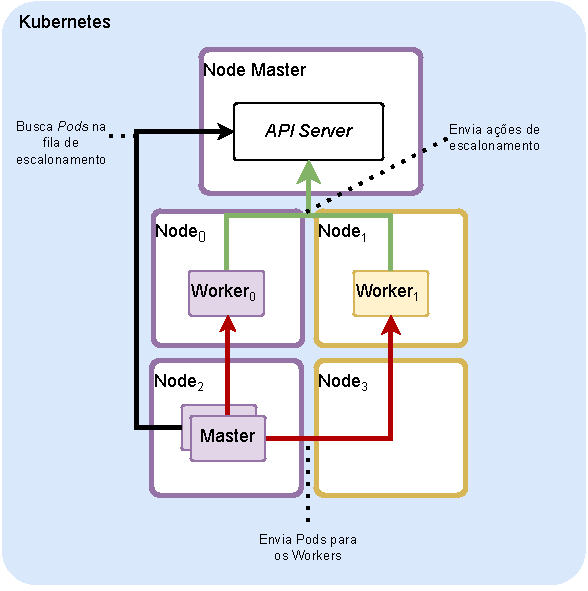
\includegraphics[width=.7\linewidth]{assets/arquitetura-worker.pdf}
	\legend{Fonte: O autor}
\end{figure}

Na figura percebe-se que as instâncias do componente \textit{Master} residem no \textit{Node$_2$}, isso se deve ao fato que as instâncias dos componentes do \ac{KMS} são conteinerizados e escalonadas pelo escalonador padrão do \textit{Kubernetes}. Logo, não é tarefa do escalonador proposto pré definir os nodes em que as próprias instâncias serão executadas, isso é tarefa do \textit{Kubernetes} por meio do escalonador padrão.

Ao utilizar o método de múltiplos escalonadores, no momento de provisionar um novo \textit{pod} para a plataforma é necessário discriminar o escalonador desejado, que é possível por meio do atributo \textit{schedulerName}. Isso é alterado facilmente no arquivo de manifesto do \textit{pod}, como ilustra a Figura \ref{fig:pod_custom_scheduler}.

\begin{figure}[h!]
	\caption{\label{fig:pod_custom_scheduler}Direcionamento do \textit{pod} para o escalonador \textit{my-scheduler}}
	\centering
	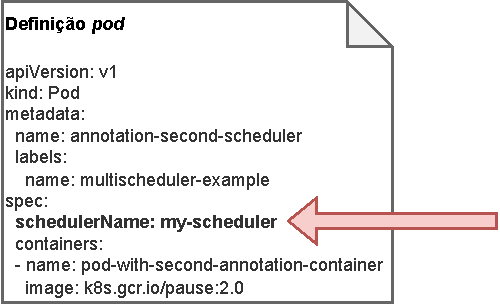
\includegraphics[width=0.6\linewidth]{assets/pod-custom-scheduler.pdf}
	\legend{Fonte: O autor}
\end{figure}

\section{Representação por Diagramas de Classes}

O diagrama de classes da proposta é visualizado pelas figuras \ref{fig:master_class_diagram} e \ref{fig:worker_class_diagram}. No diagrama do \textit{Worker} é utilizado o padrão de projeto \textit{strategy} para alternar o método de escalonamento, além disso, há também outros dois métodos -- \textit{solve} e \textit{binding}. \textit{Solve} é responsável por resolver o escalonamento de acordo com a estratégia escolhida, e \textit{binding} tem como objetivo enviar uma ordem de escalonamento para \textit{Kubernetes} utilizando a \textit{API}.

\subsection{Master}
\begin{figure}[h!]
	\caption{\label{fig:master_class_diagram}Diagrama de Classes \textit{Master}}
	\centering
	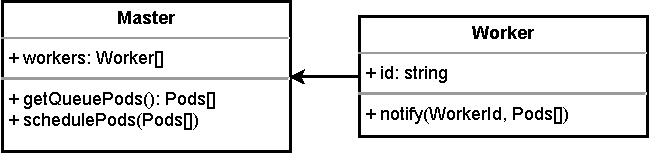
\includegraphics[width=0.65\linewidth]{assets/master-class-diagram.pdf}
	\legend{Fonte: O autor}
\end{figure}

\subparagraph{Classe \textit{Worker}:}
Representa a entidade \textit{Worker} no escopo do \textit{Master}. Em resumo, consiste em um atributo para identificação -- \textit{id} -- e um método para a comunicação de envio dos \textit{Pods} denominado \textit{notify}.

\subparagraph{Classe \textit{Master}:}
Possui uma lista de \textit{Workers} vinculados, é responsável por buscar os \textit{Pods} que estão na fila de escalonamento do \textit{Kubernetes} -- \textit{getQueuePods}. Já o método \textit{schedulePods} objetiva executar o particionamento e direcionar cada parte da fila de escalonamento para um \textit{Worker} específico.
\subsection{Worker}
\begin{figure}[h!]
	\caption{\label{fig:worker_class_diagram}Diagrama de Classes \textit{worker}}
	\centering
	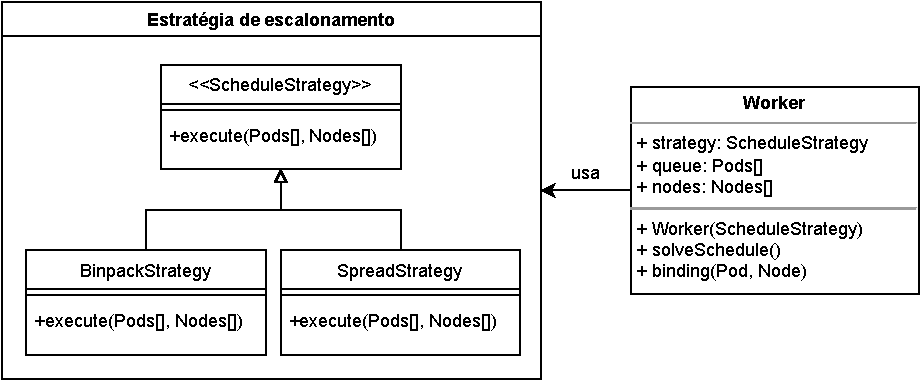
\includegraphics[width=1\linewidth]{assets/worker-class-diagram.pdf}
	\legend{Fonte: O autor}
\end{figure}

\subparagraph{Interface \textit{ScheduleStrategy}:}
Implementação do padrão de projeto \textit{Strategy}, permite intercambiar o método de escalonamento.

\subparagraph{Classe \textit{BinpackStrategy}:}
Executa o escalonamento utilizando técnica de agrupamento.

\subparagraph{Classe \textit{SpreadStrategy}:}
Executa o escalonamento utilizando técnica de espalhamento.

\subparagraph{Classe \textit{Worker}:}
Executa o escalonamento a partir da estratégia selecionada. A estratégia é escolhida no método de construção da classe \textit{Worker(ScheduleStrategy)}. Também há a especificação da fila de escalonamento representado pelo atributo \textit{queue} e dos nós -- \textit{nodes} -- que o \textit{Worker} está gerenciando. O método \textit{solveSchedule} executa o escalonamento a partir da estratégia selecionada e \textit{binding} envia ordem de escalonamento para \textit{API} do \textit{Kubernetes}.

\section{Considerações parciais}
A proposta apresentada nesse capitulo visou o desenvolvimento de um sistema distribuído, fundamentada em microsserviços, para escalonamento de contêineres em \textit{Kubernetes}. Na seção 3.1 foram confrontadas as abordagens de escalonamento oferecidas pelo \textit{Kubernetes} ao lado do \ac{KMS},  a seguir foram levantados os requisitos com objetivo de definir o escopo do projeto. As seções subsequentes explicaram o funcionamento dos componentes principais do \ac{KMS}, com ênfase na característica \textit{stateless} do \textit{Worker}. Na seção 3.4 foi demonstrada a troca de mensagens entre os sistemas, e em sequência a explicação do algoritmo de eleição do componente \textit{Master}. Por fim, foi apresentado um exemplo de implantação do \ac{KMS} em \textit{Kubernetes} e a identificação dos diagramas de classes dos componentes principais.
 





